\documentclass[10pt, conference, compsocconf]{IEEEtran}
% Set letter paper size:
\setlength{\paperheight}{11in}
\setlength{\paperwidth}{8.5in}
\usepackage[pass]{geometry}
\usepackage{amsmath}

\usepackage{color}
\usepackage{tikz}
\usetikzlibrary{arrows,positioning} 

\begin{document}
%
% --- Author Metadata here ---
%\conferenceinfo{SC'15}{'15 Austin, Texas USA}
%\CopyrightYear{2007} % Allows default copyright year (20XX) to be over-ridden - IF NEED BE.
%\crdata{0-12345-67-8/90/01}  % Allows default copyright data (0-89791-88-6/97/05) to be over-ridden - IF NEED BE.
% --- End of Author Metadata ---

\title{Increasing the Energy Efficiency of Distributed Sorting by Avoiding Communication}

\author{\IEEEauthorblockN{Hari Sundar, Saurav Muralidharan, Amit Roy, Mary Hall, Prajakta Mane}
\IEEEauthorblockA{University of Utah\\
Salt Lake City, UT\\
E-mail: \{hari, sauravm, aroy, mhall, mane\}@cs.utah.edu}
}

\maketitle
\begin{abstract}
Sorting is an essential building block for several algorithms and applications. As we ramp up to the first exascale systems, it is important to look beyond the usual metrics of performance and scalability and also consider the energy and power requirements of sorting algorithms. 
In this work we improve the energy efficiency of distributed sorting by proposing a new algorithm that avoids communication whenever possible. In addition, we analyze the most energy and power efficient sorting strategies on GPUs and Heterogeneous system architectures.
\end{abstract}

% \category{H.4}{Information Systems Applications}{Miscellaneous}
% \category{D.2.8}{Software Engineering}{Metrics}[complexity measures, performance measures]

% \terms{Theory}

% \keywords{ACM proceedings, \LaTeX, text tagging}

\section{Introduction}

Large-scale distributed sorting have focused on improving sort throughput (number of keys sorted per sec) and parallel scalability. However, for the next generation of supercomputers, additional metrics related to energy and power consumption are going to be equally if not more important. Since, sorting is entirely dominated by data movement, energy is equivalent to the total data communicated and power is proportional to the peak bandwidth utilized. This makes distributed sorting an ideal algorithm to study energy and power related optimizations. The motivation is to develop a distributed sorting algorithm that aims to minimize the overall data-movement, the peak bandwidth required without sacrificing either performance or scalability. The development of such a distributed sorting algorithm is the central contribution of this work. We propose both distributed as well as node-local strategies to achieve this goal. Our expectation is that this work will serve as guideline for the development of such energy and power efficient for a wider array of problems in the near future.

Relevance. 
 
Motivate and connect to a larger set of problems. Highlight contributions and list limitations.

\section{Background}
Keep related work here and separate from introduction. some glue text here before we go into separate subsections on the energy aspects and the algorithmic aspects of sorting.

\subsection{energy considerations on GPUs}

\subsection{Sorting Algorithms}
The design and implementation of parallel algorithms for sorting is a well studied subject. In our discussion of prior work, we focus our attention to distributed memory algorithms that have been experimentally shown to scale to large core counts and large datasets. We will also discuss related sorting algorithms (albeit not at scale) that study the energy-efficiency of sorting. We begin by a formal definition of distributed sorting.


Given an array $A$ with $N$ keys and an order (comparison) relation, we would like to sort the elements of $A$ in ascending order. In a distributed memory machine with $p$ tasks, every task is assigned an $N/p$-sized block of $A$. Upon completion, task $i$ will have the $i^{\text{th}}$ block of the sorted array. Note that the overall ordering of the keys is determined by the ordering of the tasks as well as the ordering of the keys on each task.  

\paragraph{Distributed sorting}

The most popular algorithm used in actual distributed
sort implementations is SampleSort, originally proposed by Frazer and McKellar\cite{samplesort}. Given $p$ tasks, we
reshuffle the elements of $A$ in $p$ buckets so that the all the
keys in the $i^\text{th}$ bucket are smaller (or equal) than the keys in
the $(i+1)^\text{th}$ bucket. Bucket $i$ is assigned to task $i$ and thus,
once we have shuffled $A$, each task can sort its bucket of
keys in an embarrassingly parallel manner using any local
(shared-memory-parallel) sort algorithm. The challenge is to obtain good load-balancing, i.e., ensuring that each 
task  has roughly the same number of keys, while minimizing communication costs.  

One possible way to reshuffle $A$ is to estimate the boundaries for each bucket, by selecting $p-1$ keys, which we call
``splitters''. This can be done  by sampling a
subset of keys in $A$, sorting them and selecting splitters from that set. Once these $p-1$ splitters have been
selected, a global data exchange takes place to move the original keys of every task to their correct bucket.
An additional local sort is invoked to finalize the output array. SampleSort is well understood. However, its performance is quite sensitive to the selection of splitters, which can result in load imbalance. Most importantly, the final data exchange---requiring $\mathcal{O}(p^2)$ messages---can congest the network. As a result SampleSort may scale 
suboptimally, especially when the communication volume approaches the available hardware limits \cite{hyksort}.

Parallel HistogramSort~\cite{kale93,solomonik10} is
a variant of SampleSort that efficiently estimates the splitters. The authors presented
one of the largest distributed comparison sort runs (32K cores on
BG/P) with $46\%$ efficiency. The algorithm overlaps communication
and computation in all stages. During the splitter estimation
stage, the iterative estimation of the ranks of the splitters is
combined with partial local sorting of the data, by using the
splitter candidates as pivots for quicksort. Once the splitters
are estimated, the communication of data is staged and overlapped
with local merging. In~\cite{solomonik10} the best throughput was
obtained on 16,384 cores of Jaguar XT4 at ORNL for 8M (64-bit) keys
per core; the sort took 4.3 seconds achieving a in-RAM throughput of
14.4TB/min. 

CloudRAMSort \cite{kim12} demonstrated good scalability on 256 nodes with shared memory
parallelism using {\texttt pThreads} and SIMD vectorization. The
best results are for sorting 1TB of data (10byte key + 90byte
record) in 4.6 secs achieving an in-RAM throughput of 12.6 TB/min. They
use a variant of Histogram Sort~\cite{kale93}, where the
samples are iteratively computed (in parallel) in order to guarantee
a minimum quality of load-balance. Additionally, the communication of the records is split into two parts by first communicating the keys followed by the values overlapped with the merging of the keys. 

In recent work \cite{hyksort}, we have addressed the scalability of sorting on very large clusters. Hyksort\cite{hyksort} is an extension of quicksort on a Hypercube \cite{wagar87} to a $k$-ary Hypercube along with an efficient parallel (median) selection algorithm. 

\paragraph{Energy-efficient and GPU sorting}
mention the general approaches. 

\paragraph{Code variant tuning}
Apart from Nitro~\cite{muralidharan:2014},
several programmer-directed autotuning frameworks support
tuning of code/algorithmic variants.
Petabricks~\cite{PetaBricks} 
supports user specification of \textit{transforms} that
are analogous to functions. Transforms are automatically
composed together to form hybrid algorithms using a compiler
framework and an adaptive algorithm~\cite{increa11}. Petabricks, however,
implicitly tunes variants for the size of the input data set. Ding et
al.~\cite{ding:2015} propose extensions to the PetaBricks language to
enable support for tuning based on arbitrary input features.

\paragraph{Multi-objective optimization}

\section{Distributed Sorting}
\label{sec:dsort}

Large-scale distributed sorting, such as those discussed in \S\ref{sec:bg-dist}, have focused on improving sort throughput (number of keys sorted per sec) and parallel scalability. Since, sorting is entirely dominated by data movement, energy is equivalent to the total data communicated and power is proportional to the peak bandwidth utilized. This motivates us to design an algorithm that minimizes the peak-bandwidth requirement as well the overall data communicated. In this section, we first look at the theoretical arguments in this direction, leading to the actual arguments. 

In \cite{hyksort}, we proposed a variant of HyperQuicksort\cite{wagar87} that allowed us to control the algorithm behavior by adjust a parameter $k$. Selecting $k=2$ made the algorithm behave as HyperQuicksort, whereas selecting $k=p$ resulted in behavior similar to Samplesort. The bandwidth term for the algorithm is,
\begin{equation}
  \label{eq:bw}
    k \frac{\log^2 p}{\log k} + \frac{N}{p}.
\end{equation}   
Ignoring the $N/p$ term, we can see that for Samplesort($k=p$) the bandwidth required is $\mathcal{O}(p\log^ p)$, whereas it is only $\mathcal{O}(\log^ p)$ for Hyperquicksort. So clearly, Hyperquicksort is preferable from the bandwidth (and therefor power) perspective. An added benefit is that Hyperquicksort only sends $\mathcal{O}(p)$ message at each stage as opposed to $\mathcal{O}(p^2)$ for Samplesort. While Hyperquicksort does communicate $\mathcal{O}(n\log n)$ data, as compared with $\mathcal{O}(n)$, it's overall performance and scalability is comparable to Samplesort\cite{hyksort}. It is not possible to reduce the bandwidth term for Samplesort, so we modify Hyperquicksort to reduce the amount data it needs to communicate. This is achieved by selectively changing the task-role instead of moving data between tasks. We call this algorithm {\sc SwapRankSort}. This is in principle similar to moving the computation to the data instead of moving the data to the computation. We now elaborate on {\sc SwapRankSort}.

\subsection{{\sc SwapRankSort}}

During each stage of Hyperquicksort, each task exchanges data with another task whose {\em rank}\footnote{a unique identifier assigned to each task.} differs from its own at bit-$k$, where $k$ is the current stage of Hyperquicksort. How much data is exchanged between the tasks depends on the distribution of local-data on each task and the global median of the data (at this level). Analogous to quicksort, the lower-ranked task retains the keys smaller than the median (pivot) and the higher-ranked task retains the higher keys. Depending on the local-distribution of the keys, all the keys ($N/p$) might be exchanged between the tasks. In {\sc SwapRankSort}, we propose a minor modification, where we evaluate the cost of exchanging data for the default case as well as if the ranks of the two tasks were swapped. A swap simply means that a task that would have retained the smaller keys will now retain the larger keys. Clearly that maximum amount of data exchanged in this case is $N/2p$. 

Given that we run this in a distributed setting implies that even a single pair of tasks having a skewed distribution will cause the overall algorithm to exhibit poor performance. Also note that in case of uniformly distributed (amongst the tasks, independent of the data distribution) keys, {\sc SwapRankSort} performs the same as Hyperquicksort with no tasks swapping ranks. The actual swapping of the ranks takes place at the end of each stage when we split the communicator. This is a step that is needed for Hyperquicksort as well, so there is no significant overhead to swapping ranks. 

\begin{figure}
  \begin{center}
  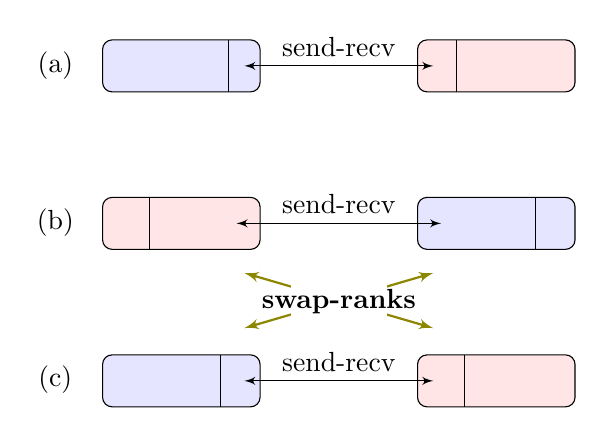
\begin{tikzpicture}
      \draw[fill=blue!10,rounded corners=.8ex] (0,0) rectangle +(2,0.66);
      \draw[fill=red!10,rounded corners=.8ex] (4,0) rectangle +(2,0.66); 
      
      \draw (1.6,0) -- (1.6,0.66);
      \draw (4.5,0) -- (4.5,0.66);
      
      %\path[<->] (2.2,0.33) edge node[above] {no swap} (3.8,0.33);
      
      \path[latex'-latex'] (1.8,0.33) edge node[above] {send-recv} (4.2,0.33);
      
      \node at (-0.6,0.33) {(a)};
      \node at (-0.6,-1.66) {(b)};
      \node at (-0.6,-3.66) {(c)};
      
      \path[latex'-latex',thick,olive] (1.8,-2.3) edge (4.2,-3);
      \path[latex'-latex',thick,olive] (4.2,-2.3) edge (1.8,-3);
      
      \draw[fill=white,white] (2.4,-2.9) rectangle +(1.2,0.5);
      
      \node at (3.0,-2.66) {\bf swap-ranks};
      
      \begin{scope}[shift={(0,-2)}]
        \draw[fill=red!10,rounded corners=.8ex] (0,0) rectangle +(2,0.66);
        \draw[fill=blue!10,rounded corners=.8ex] (4,0) rectangle +(2,0.66); 
        
        \draw (0.6,0) -- (0.6,0.66);
        \draw (5.5,0) -- (5.5,0.66);
        
        \path[latex'-latex'] (1.7,0.33) edge node[above] {send-recv} (4.3,0.33);
        
      \end{scope}
      
      \begin{scope}[shift={(0,-4)}]
        \draw[fill=blue!10,rounded corners=.8ex] (0,0) rectangle +(2,0.66);
        \draw[fill=red!10,rounded corners=.8ex] (4,0) rectangle +(2,0.66); 
        
        \draw (1.5,0) -- (1.5,0.66);
        \draw (4.6,0) -- (4.6,0.66);
        
        \path[latex'-latex'] (1.8,0.33) edge node[above] {send-recv} (4.2,0.33);
        
      \end{scope}

  \end{tikzpicture}
  \end{center}
  \caption{\label{fig:swaprank} Illustration of the central idea behind {\sc SwapRankSort}. In (a) the distribution of the keys results in the tasks exchanging a small number of keys. Ranks are not swapped in this case and the program behavior is the same as Hyperquicksort. In (b), we illustrate the case where the smaller ranked task (in blue) has a large number of keys greater than the pivot, and the higher ranked task(red) has a large number of keys smaller than the pivot. This results in a lot of data exchange. In (c), we illustrate {\sc SwapRankSort} where the tasks swap ranks and exchange the smaller set of keys. }
\end{figure} 

\section{Energy-Efficient Node Sorting}
The previously-described distributed sorting algorithm relies
on a node-level sort of the subset of data assigned to each node at 
each stage of the sort.  This section describes how we arrive 
at a node-level sorting algorithm that is both energy efficient and
high performance.  

\subsection{Overview of Approach}
We first present an overview of the node-level sorting approach, 
looking at factors such as resource selection in a heterogeneous platform, 
sorting algorithms, and how we extend an existing framework for performance
optimization to also take into account energy and power consumption.

\vspace*{.1in}

\noindent
{\bf GPU vs. Parallel CPU Sorting.}
{\color{red}Establish that GPU is highest performing and most energy efficient for node sort.
Show performance (and possibly energy) 
difference for both Titan and Jetson compared with OpenMP?}  

\vspace*{.1in}

\noindent
{\bf Sorting algorithms as code variants.}
It is well established that the best algorithm for sorting
is dependent on input data set (type, size and distribution), target 
architecture and implementation details.   Therefore, the best-performing
and most energy-efficient implementation cannot
be determined until run time without a prior knowledge of these factors.
We refer to different sorting algorithms or implementations
as \emph{code variants}.  
A number of techniques for code variant selection and algorithm
selection have been described in the literature~\cite{algsel}, and our approach
will rely on recent advancements in this area as described in this section.
 
In this paper, we select among two algorithms to use for
the node-level sort.  
\begin{itemize}
\item \emph{Merge Sort:}
Merge Sort sorts a list of data by 
recursively splitting the list in half, sorting each half,
and then merging the two sorted lists together.
The Merge Sort implementation we use is
part of the ModernGPU~\cite{modernGPU} library of GPU
primitives.  
\item \emph{Radix sort:}
Radix Sort achieves a sorted list by grouping keys by individual digits  
that have the same position and value.
The Radix sort implementation is provided in CUB~\cite{cub}. 
\end{itemize}
{\color{red} May want to also say when one might be preferable to another.}

\vspace*{.1in}

\noindent
{\bf Managing energy and power on the GPU.} 
We use two mechanisms to adjust energy and power usage on the GPU.  
We can monitor energy or power usage for each of the two 
sort algorithms, and together with performance measurements,
select the preferred algorithm.  In addition, the target Nvidia GPUs
allow adjusting of the clock frequency, or frequency of the memory
bus.  Through monitoring energy or power at different frequency
settings, we can select the preferred frequency(ies).  

Since we would prefer an implementation that is both high performing and
power or energy efficient, we must develop a \emph{selection 
criteria} that considers multiple optimization goals in selecting the
node-level sorting algorithm.
%employ multi-objective tuning, which selects an 
%implementation according to both its performance and its energy usage or
%peak power requirements.  
The next subsection will describe
a number of different selection criteria we explore in this paper
and their overall impact on performance, energy and power.

\vspace*{.1in}

\noindent
{\bf Code variant selection using Nitro.}
The system described in this paper used for code variant
selection extends
the Nitro autotuning framework~\cite{muralidharan:2014}.
Nitro provides a library interface that permits expert programmers to
express code variants along with meta-information that aids
the system in selecting among the set of variants at runtime.
Figure~\ref{fig:overview} illustrates the approach in Nitro.  
A learning algorithm -- Support Vector Machine (SVM) classifier by default -- co
nstructs a 
code variant selection
model on the target architecture as a result of an offline training phase on the
 same architecture.
For each architecture, training data has the form
$\{(\mathbf{x}_1, y_1), \hdots, (\mathbf{x}_M, y_M)\}$, where
each $\mathbf{x}_i$ represents an input feature vector and each
$y_i$ represents the best variant for that input.
When presented with a new, unseen input at runtime, the model
predicts the best variant to use. 
For sort, prior work has used data type, data set size and presortedness
as features~\cite{muralidharan:2014}.  In this paper,
we omit presortedness, and replace it with the distribution
of key values.  These three features are available when the
sort is invoked, and can be used in consulting a model for code
variant selection at run time.
In this paper, we extend Nitro in two ways: (1) we treat 
different clock frequencies as code variants, in addition to the
different sorting algorithms; and, (2) the model is trained
using both performance and energy/power data, according to the 
selection criteria outlined in the next subsection.

\subsection{Code Variant Selection Criteria}
Application tuning that looks at multiple optimization criteria
is referred to as \emph{multi-objective tuning}.
A challenge with multi-objective tuning is that the solution must encompass
a tradeoff space between different optimization objectives.  Any 
solution among the \emph{Pareto frontier} is valid; these points are ones
for which there is no other solution that has better metrics among
all the set of objectives.
{\color{red} CLEAN UP AND ADD CITATIONS!!!
Techniques for multi-objective tuning resolve this selection in several
ways:
(1) treat one objective as independent (e.g., an equivalence class
as in PetaBricks paper);  (2) weight one objective above others; 
(3) ask users; (4) use heuristics to drive optimization; or, (5) come up with combined metric.}

In this paper, we have chosen to use a set of fairly standard combined metrics.
We explore which leads to the best reduction in energy or power with the least
impact on performance.  These metrics are as follows: 
\begin{itemize}
\item MKeys per Joule: {\color{red} Define}
\item MKeys$^2$ per Joule: {\color{red} Define}
\item MKeys per Watt: {\color{red} Define}
\item MKeys$^2$ per Watt: {\color{red} Define}
\end{itemize}
These were selected because they capture the relationship between throughput
and energy or power.  Further, it is straightforward to build a model 
for code variant selection by consolidating on a single metric.
In our experiments we will show {\color{red} some indication that this works well.}

\section{Experimental Methodology}

This section describes the input data for sort and the
three target architectures used in our experiment.

\paragraph{Input Data}
As the performance of sort is dependent on its input data, we 
use a variety of data types, distributions and sizes in our experiments.
We consider XXX data types: 
integer, long integer, float, double, {\color{red} fill in
the rest.}
The distribution of key values 
includes a uniform distribution, a Gaussian distribution, 
{\color{red} fill in
the rest.}
Sizes are motivated by each experiment and the capacity of the
target architecture.  {\color{red} For Titan, ...  
For K20c ... For Jetson ...  Perhaps this goes in the results section.}

\paragraph{Titan (ORNL)} 
We are interested in 
achieving scalable energy efficiency for distributed
sorting on supercomputers, and therefore the target architecture is the
Titan system at Oak Ridge.  Titan has 
{\color{red}... CPUs ... GPUs ...  compiler/OpenMP/MPI installations?}
We would like to measure performance on the GPUs on Titan, but encountered
an obstacle in the software installation.  
The CUDA version used on Titan is CUDA XXX, which is out-of-date with respect to
sorting implementations we are using.  We are also unable to measure
power and energy in the same way on Titan as on the other platforms.
Therefore, we will focus our
Titan experiments on using the OpenMP implementation of sorting, and focus
data gathering on the communication and scaling aspects of our optimizations.
We will then extrapolate
Titan GPU results using other representative clusters.

%\noindent
%{\bf K20 cluster.}
%{\color{red} This is the SCI cluster.  Omit if we don't have results on it.}

\paragraph{NVIDIA K80 Standalone GPU}
For the node-level experiments, we used an NVIDIA K80 (Kepler 
generation) standalone GPU.
It has 26 GPU streaming multiprocessors, for a total of 4992 cores, 
and 24 GBytes of memory.

The K80 supports 25 core clock frequency settings ranging from 562 Mhz to 875 Mhz
in 13 Mhz increments.
It supports two memory frequencies as well, 
but we do not adjust memory frequency in these experiments 
because the lower memory frequency of 324 Mhz
is far lower than peak of 2505 Mhz
and is therefore going to perform poorly in a bandwidth-limited
algorithm such as sort.
For frequency adjustments and energy and power measurements, we use the NVML
API~\cite{} from NVIDIA. The K80 also uses a mechanism called \textit{AutoBoost} to dynamically
vary clock frequencies to fill available power headroom. We disable this feature
for more consistent data collection.

\paragraph{Jetson TK1 Cluster}
We also measured performance of distributed sorting on an NVIDIA 
Jetson TK1 cluster; the nodes of the Jetson are low-power and lightweight,
consisting of a single GPU streaming multiprocessor (Kepler generation)
with 192 cores, and 
four-plus-one ARM cores, where the fifth ARM core is used as a master processor.
The nodes have a unified DRAM of 2 GBytes, which is shared between CPUs and
GPUs, and separate cache structures for CPU and GPU.
The cluster we use in this experiment has 16 nodes, and
the nodes are connected with {\color{red} ... network details.}
The software installation uses CUDA 6.5, nvcc compiler version 6.5.35,
MPI version 1.6.5, and OpenMP version 3.1.

The power and energy reported for
Jetson are physical measurements  
using the Yokogawa WT310 digital multimeter.
We measure the voltage drop across a known precision resistance in series with the device under test (DUT).
With a known resistance and measured voltage on that resistance,
the current can be obtained with the equation $I=V/R$.
Here, the resistance is 0.020 Ohms with a 1\% variation.
To determine the power, we use the equation $P=IV$, where $I$ is the value calculated above, and $V$ is 12.19V.
The Jetson has 14 core clock frequencies ranging from 72MHz to 852MHz,
and twelve memory frequencies from 12.75MHz to 924MHz;
since collecting physical measurements 
on all 1728 combinations of core/memory frequency per data set would 
be prohibitively time-consuming, we only varied core frequencies for our experiments.

While not capable of the high GPU performance of the K80
since it has only one-thirteenth of the SMs,
the Jetson cluster looks to the future of high-performance and 
embedded GPU platforms. Support for unified memory allows us to look 
at power and energy without the data movement required to copy
from CPU to GPU, and the large number of frequency adjustments
allow us to examine how the large number of degrees of freedom
in energy management impacts energy, power and performance in 
code variant selection. 

\section{Experimental Results}

{\color{red} Things to answer.}
\begin{itemize}
\item Are different algorithms affected differently by frequency adjustment?
\item How does frequency affect performance/energy/power?
\item End with SCI cluster and Titan results, and extrapolate from prior 
measurements.
\end{itemize}


\begin{table*}[tb]
  \begin{center}
  %\resizebox{0.95\textwidth}{!}{
  \begin{tabular}{| l | r | r | r | r | r | r | r |}
  \hline
  \textbf{Variant} & \textbf{Performance} & $\mathbf{\frac{Throughput}{Energy}}$ & $\mathbf{\frac{Throughput}{(Energy)^2}}$ & $\mathbf{\frac{(Throughput)^2}{Energy}}$ & $\mathbf{\frac{Throughput}{Power}}$ & $\mathbf{\frac{Throughput}{(Power)^2}}$ & $\mathbf{\frac{(Throughput)^2}{Power}}$ \\ \hline
  \textbf{Merge Sort} & 0 & 0 & 0 & 0 & 0 & 0 & 0 \\ \hline
  \textbf{Radix Sort} & 0 & 0 & 0 & 0 & 0 & 0 & 0 \\ \hline
  \end{tabular}
  %}
  \end{center}
  \caption{Distribution of variant selections across inputs}
  \label{tab:ss}
\end{table*}


\section{Discussion}
Discuss results and what the key findings are and what it means for future architectures.


%ACKNOWLEDGMENTS are optional
%\section{Acknowledgments}
%Thank Christopher Strong, nvidia?, Funding agencies.


%
\bibliographystyle{IEEEtran}
\bibliography{esort,nitro,tuning} 

%\balancecolumns % GM June 2007
% That's all folks!
\end{document}
